\documentclass[8pt]{beamer}

%%%%%%%%%%%%
% PACKAGES %
%%%%%%%%%%%%

% kek 
\usepackage[T1]{fontenc} % Use 8-bit encoding that has 256 glyphs
\usepackage[utf8]{inputenc} % For Spanish characters
\usepackage[english]{babel} % USEnglish localization
% =========== General Formatting =============
\usepackage{microtype} % Slightly tweak font spacing for aesthetics
\usepackage{fancyhdr} % Allows for nice header and footer
\usepackage{appendix} % Enables appendices
\usepackage{enumerate} % Custom numerate, useful for i,ii,iii... I,II,III...
% \usepackage{hyperref} % For hyperlinks in the PDF
\usepackage{extramarks} % 
\usepackage{fontawesome} % For web icons

% =============== Math ===============
\usepackage{amsmath} % Standard math packages
\usepackage{amsthm} % Math Theorems
\usepackage{amssymb} % Math Symbols
\usepackage{amsfonts} % Math Fonts
\usepackage{mathtools} % Extra math tools such as PairedDelimiter
\usepackage{upgreek} % Nice sigma => \upsigma
\usepackage{array} % Enables array features
\usepackage{siunitx} % For SI Unit easy formatting
\usepackage{dsfont} % For math. indicators

% =============== Figures ===============
\usepackage{float} % Float features
\usepackage{wrapfig} % Al­lows fig­ures or ta­bles to have text wrapped around them
\usepackage{tikz} % Diagram and figure creation and rendering
% =============== Tables ===============
\usepackage{booktabs} % Horizontal rules in tables
\usepackage{float} % Required for tables and figures in the multi
\usepackage{multirow} % Combined rows in tables
\usepackage{multicol} % Combined columns in tables
\usepackage{colortbl} % Color cells
%\usepackage{longtable} % Tables than span multipages

% =============== Bibliography ==========
\usepackage{natbib} % Lots of useful versions of \cite

% % =============== Listings ============
\usepackage{listings} % Main package for inserting code
\usepackage[scaled]{beramono} % For using the beramono font
% % =============== Algorithms ===============
\usepackage[linesnumbered,lined,boxed,commentsnumbered]{algorithm2e} % Allows for algorithm description
\usepackage[noend]{algpseudocode}
% =============== Other ===============
\usepackage{datetime} % Date-Time formatting
\usepackage{ulem} % For strikethrough text \st{}
\usepackage{textcomp} %Text Com­pan­ion fonts

\usepackage{pdfpages} % Insert pdfs
\usepackage{lipsum} % Used for inserting dummy 'Lorem ipsum' text into the template
% \usepackage[space]{grffile} % insert files with spaces
\usepackage{pdflscape} % Individual horizontal pages
\usepackage[many]{tcolorbox} % Color boxes for comment
%\usepackage{xargs} % Expanded arguments features
%\usepackage{fix-cm} % Computer-Modern at arbitrarysizes
%\usepackage{eurosym} % Eurosymbol

% Thick strike out
\newcommand{\cancelled}[1]{%
    \renewcommand{\ULthickness}{3pt}%
       \sout{#1}%
    \renewcommand{\ULthickness}{.4pt}% Resetting to ulem default
}

\newcommand{\done}[1]{\sout{#1}}

% derivatives
\newcommand{\dderiv}[2]{\frac{\mathrm{d}}{\mathrm{d}#2} (#1)}

% partial derivatives
\newcommand{\pderiv}[2]{\frac{\partial #1}{\partial #2}}
\newcommand*{\pd}[3][]{\ensuremath{\frac{\partial^{#1} #2}{\partial #3}}}

% Integral dx
\newcommand{\dx}{\mathrm{d}x}

% Evaluation operator
\newcommand*{\at}[2]{\Big|_{#1}^{#2}}

% Probability macros
% Variance
\newcommand{\Var}{\mathrm{Var}}
% Covariance
\newcommand{\Cov}{\mathrm{Cov}}
% Bias
\newcommand{\Bias}{\mathrm{Bias}}
% Probability
\newcommand*{\prob}[1]{\ensuremath{\mathbb{P}\left[#1\right]}}
\newcommand*{\expectation}[1]{\ensuremath{\mathbb{E}\left[#1\right]}}
\newcommand*{\variance}[1]{\ensuremath{\mathbb{V}\left[#1\right]}}
% Indicator function of an event
\newcommand*{\ind}[1]{\ensuremath{\mathds{I}_{\left[#1\right]}}}

% Optimization macros
\DeclareMathOperator{\dom}{Dom}
\DeclareMathOperator{\diag}{Diag}
\DeclareMathOperator{\prox}{prox}
\DeclareMathOperator*{\proj}{Proj}
\DeclareMathOperator*{\sign}{sign}
\DeclareMathOperator*{\argmax}{argmax}
\DeclareMathOperator*{\argmin}{argmin}

\newcommand*{\pdef}{\ensuremath{\mathbb{S}_{++}}}
\newcommand*{\psdef}{\ensuremath{\mathbb{S}_{+}}}

%% \mathbb symbols
\DeclareMathOperator{\E}{\mathbb{E}}
\DeclareMathOperator{\A}{\mathbb{A}}
\DeclareMathOperator{\B}{\mathbb{B}}
\DeclareMathOperator{\R}{\mathbb{R}}
\DeclareMathOperator{\C}{\mathbb{C}}
\DeclareMathOperator{\X}{\mathbb{X}}
\DeclareMathOperator{\N}{\mathbb{N}}
\DeclareMathOperator{\Q}{\mathbb{Q}}
\DeclareMathOperator{\V}{\mathbb{V}}

%% \mathcal symbols
\DeclareMathOperator{\RR}{\mathcal{R}}
\DeclareMathOperator{\PP}{\mathcal{P}}
\DeclareMathOperator{\NN}{\mathcal{N}}
\DeclareMathOperator{\CC}{\mathcal{C}}
\DeclareMathOperator{\FF}{\mathcal{F}}
\DeclareMathOperator{\YY}{\mathcal{Y}}
\DeclareMathOperator{\XX}{\mathcal{X}}
\DeclareMathOperator{\LL}{\mathcal{L}}

%% \tilde symbols
\newcommand{\tbeta}{\tilde\beta}
\newcommand{\tgamma}{\tilde\gamma}

%% \hat symbols
\newcommand{\hbeta}{\hat{\beta}}
\newcommand{\hgamma}{\hat{\gamma}}
\newcommand{\hxi}{\hat{\xi}}

% limit arrow "goes to"
\newcommand{\goto}{\rightarrow}

% text above math symbol
\newcommand{\textabove}[2]{\mathrel{\overset{\makebox[0pt]{\mbox{\normalfont\tiny #1}}}{#2}}}

% Big O
\newcommand{\bigo}{{\mathcal O}}

% 1/2
\newcommand{\half}{\frac{1}{2}}
% 1/2
\newcommand{\halfof}[1]{\frac{#1}{2}}

% Real numbers
\newcommand\reals{{{\rm l} \kern -.15em {\rm R} }}

% Complex numbers
\newcommand\complex{{\raisebox{.043ex}{\rule{0.07em}{1.56ex}} \hskip -.35em {\rm C}}}

% Matrix functions
\DeclareMathOperator{\trace}{Tr}

% matrix environment for vectors or matrices where elements are centered
\newenvironment{mat}{\left[\begin{array}{ccccccccccccccc}}{\end{array}\right]}
\newcommand\bcm{\begin{mat}}
\newcommand\ecm{\end{mat}}

% matrix environment for vectors or matrices where elements are right justified
\newenvironment{rmat}{\left[\begin{array}{rrrrrrrrrrrrr}}{\end{array}\right]}
\newcommand\brm{\begin{rmat}}
\newcommand\erm{\end{rmat}}

% for left brace and a set of choices
\newenvironment{choices}{\left\{ \begin{array}{ll}}{\end{array}\right.}
\newcommand\when{&\text{if~}}
\newcommand\otherwise{&\text{otherwise}}
% sample usage:
%  \delta_{ij} = \begin{choices} 1 \when i=j, \\ 0 \otherwise \end{choices}

% For equations: first argument is a label, second is the equation 
\newcommand{\eql}[2]{\begin{equation}\label{eq:#1}\begin{split}#2\end{split}\end{equation}}
% Or just the equation 
\newcommand{\eq}[1]{\begin{equation}\begin{split}#1\end{split}\end{equation}}

% some useful macros for finite difference methods:
\newcommand\unp{U^{n+1}}
\newcommand\unm{U^{n-1}}
\newcommand\un{U^{n}}

% paired parenthesis
\DeclarePairedDelimiter\pa{(}{)}%
\DeclarePairedDelimiter\bra{[}{]}%
\DeclarePairedDelimiter\curly{\{}{\}}%
\DeclarePairedDelimiter\abs{\lvert}{\rvert}%
\DeclarePairedDelimiter\norm{\lVert}{\rVert}%
\DeclarePairedDelimiter\floor{\lfloor}{\rfloor}%
\DeclarePairedDelimiter\ceil{\lceil}{\rceil}%

% colorful box (for putting around equality signs etc)
\newtcbox{\mywboxtext}[1]{on line,colback=white,colframe=#1,size=fbox,arc=3pt,boxrule=0.8pt}
\newcommand{\boxaround}[2]{\mywboxtext{#2}{$#1$}}





% \usetheme[progressbar=frametitle]{metropolis}
\usepackage{appendixnumberbeamer}


% PRESETS OF PACKAGES AND MATH %

\usepackage{xspace}
\usepackage{caption}
\usepackage{subcaption}
\newcommand{\themename}{\textbf{\textsc{metropolis}}\xspace}
\newcommand{\ouralgo}{\ensuremath{\mathcal{MSR}3}}
\title{A Relaxation Approach to Feature Selection \newline for Linear Mixed-Effects Models}
\date{\today}
\author{Aleksei Sholokhov, James V. Burke, Peng Zheng, Damian Santomauro, and Aleksandr Aravkin}
\titlegraphic{
\includegraphics[width=0.5\textwidth]{Figures/UW_amath.pdf}\hspace{3em}
\includegraphics[height=1cm]{Figures/IHME_Logo.jpg}}

\begin{document}

\maketitle

\section{Relaxed for Linear Mixed-Effect Models}
\subsection{Mixed-Effects Models}
\begin{frame}{Mixed-Effect Models}

\begin{itemize}
	\item Used for analyzing \textbf{combined data} across a range of \textbf{groups}.
	\item Use covariates to separate the \textbf{population variability} from the \textbf{group variability}.
	\item \textbf{Borrow strength} across groups to estimate key statistics. % when data within units are sparse or highly variable.
	\item Often seek \textbf{sparse models} that only use \textbf{most informative} covariates. 
\end{itemize}

\begin{figure}
	\centering
	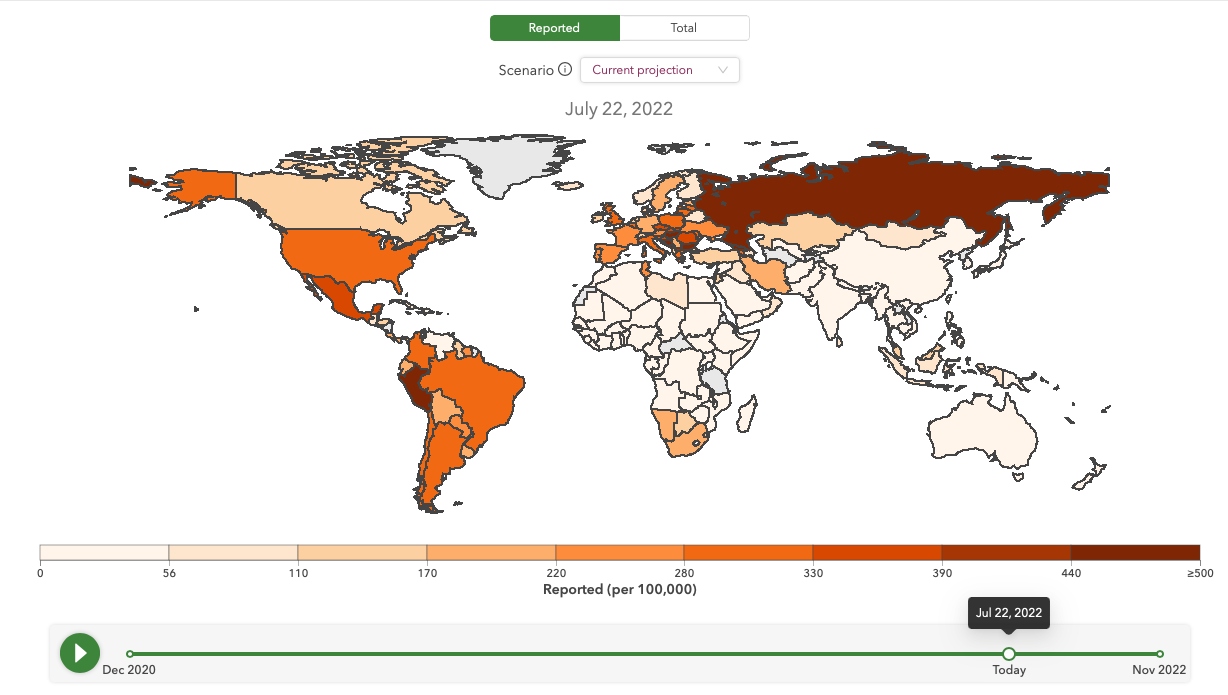
\includegraphics[width=0.8\textwidth]{Figures/ihme_predictions.png}\footnote{Picture is taken from \href{covid19.healthdata.org}{covid19.healthdata.org} }
\end{figure}

\end{frame}

\begin{frame}{Linear Mixed-Effect (LME) Models}

	Dataset: $m$ groups $(X_i, Z_i, y_i),\quad i = 1, \dots m$, each has $n_i$ observations
	\begin{itemize}
		\item 	$X_i \in \R^{n_i \times p}$ -- group $i$ design matrix for fixed features
		\item 	$Z_i \in \R^{n_i \times q}$ -- group $i$ design matrix for random effects
		\item 	$y_i \in \R^{n_i}$ -- group $i$ observations  
	\end{itemize}
	

	\begin{columns}[T,onlytextwidth]
    \column{0.5\textwidth}
	 \centering Standard Linear Regression:
   	\begin{figure}
   		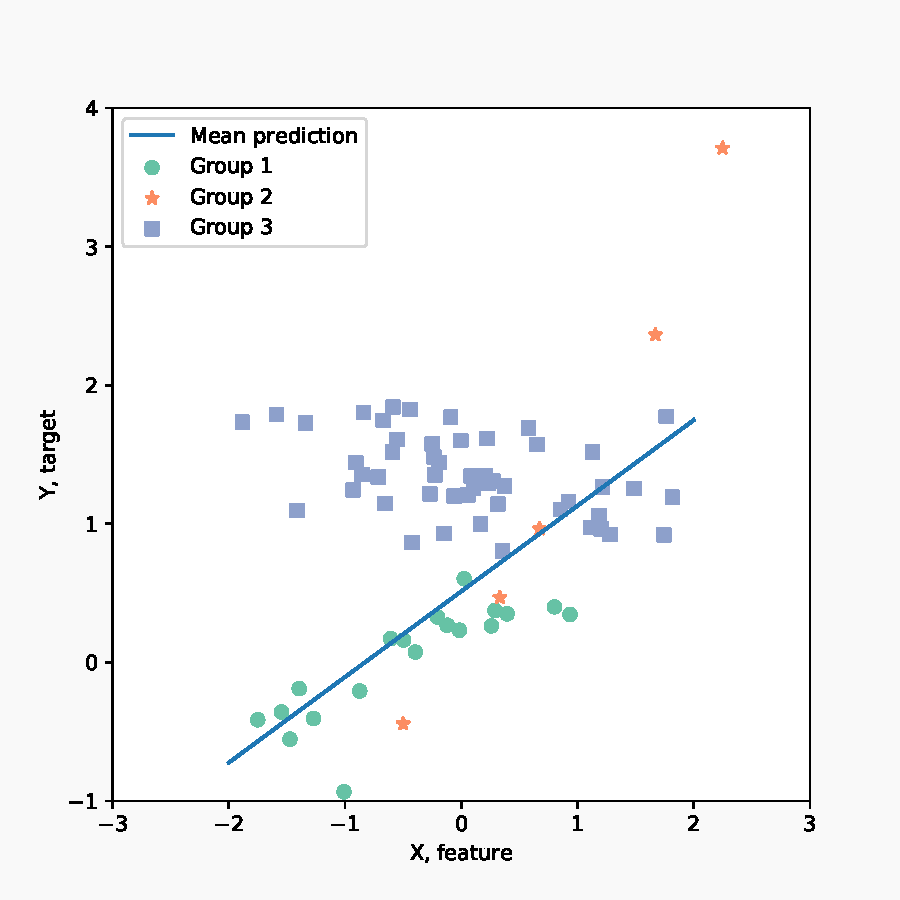
\includegraphics[width=0.9\textwidth]{Figures/lme_example_mean_prediction}
   	\end{figure}
   	\[
   		y = X\beta + \varepsilon, \quad \varepsilon \sim \NN(0, \Lambda) 
   	\]

   	
    \column{0.5\textwidth}
    	\centering  Linear Mixed-Effect Model:
   	\begin{figure}
   		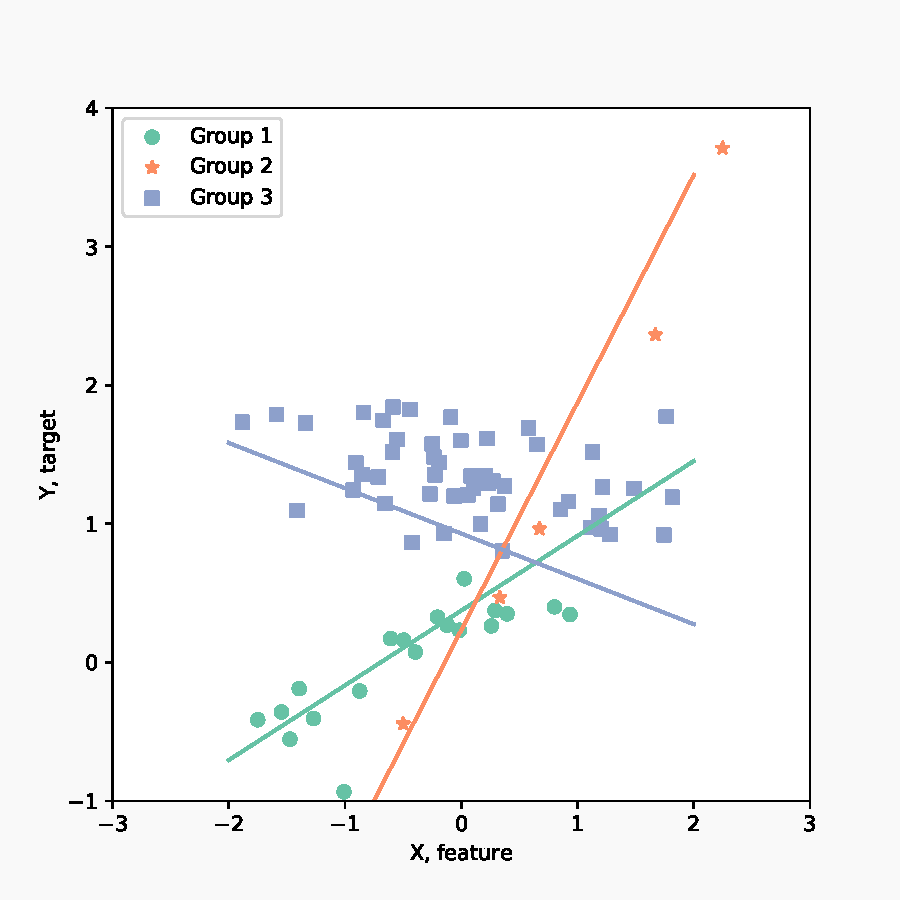
\includegraphics[width=0.9\textwidth]{Figures/lme_example_random_prediction}
   	\end{figure}
   	   		\[
   		\begin{split}
   			y_i & = X_i\beta + {\color{red}Z_i u_i} + \varepsilon_i, \quad \varepsilon_i \sim \NN(0, \Lambda_i) \\
   			{\color{red} u_i} & {\color{red}\sim \NN(0, \Gamma)}
   		\end{split}
   		\]

   	
  \end{columns}
\end{frame}

\begin{frame}{Notation}
	\eq{
   		y_i & = X_i\beta + Z_iu_i + \varepsilon_i \quad i = 1\dots m \\
   		\varepsilon_i & \sim \NN(0, \Lambda_i) \\
   		u_i & \sim \NN(0, \Gamma)
   	}   	
   	
   	\begin{itemize}
   		\item $p$ -- number of fixed features, $q$ -- number of random effects.
   		\item $\beta \in \R^p$ -- fixed effects, or mean effects
   		\item $u_i \in \R^q$ -- random effects
   		\item $\Gamma \in \R^{q \times q}$ -- covariance matrix of random effects, often $\Gamma = \diag{(\gamma)}$
   		\item $\varepsilon_i \in \R^{n_i}$ -- observation noise
   		\item $\Lambda_i \in R^{n_i \times n_i}$ -- covariance matrix for noise
   	\end{itemize}
   	Unknowns: $\beta$, $u_i$, $\gamma$, sometimes $\Lambda_i$.
\end{frame}

\begin{frame}{Likelihood for Mixed Models}
Negative log-likelihood:
\eq{
	\label{eq:lmm_objective}
	\mathcal{L}(\beta, \gamma) & = \sum_{i = 1}^m \half(y_i - X_i\beta)^T(Z_i\Gamma Z_i^T + \Lambda_i)^{-1}(y_i - X_i\beta) + \\ & + \half\log{\det{\pa{Z_i \Gamma Z_i^T + \Lambda_i}}}, \quad \Gamma = \diag{(\gamma)}
	}
Maximum likelihood estimates for $\beta$ and $\gamma$ solve the problem:
\eq{
	\mathcal{LME} \quad \min_{\beta \in \R^p,\, \gamma \in \R^{q}_+} \LL(\beta, \gamma)
}

To select covariates we add a sparsity-promoting regularizer $R(\beta, \gamma)$
\eq{
	\mathcal{FS-LME} \quad \min_{\beta \in \R^p,\, \gamma \in \R^{q}_+} \LL(\beta, \gamma) + R(\beta, \gamma)
}

\begin{itemize}
	\item $\LL(\beta, \gamma)$ is smooth on its domain, quadratic w.r.t. $\beta$ and $\bar\eta$-weakly-convex w.r.t. $\gamma$.
	\item $R(\beta, \gamma)$ is closed, proper, convex, with easily computed \textit{prox operator}
\end{itemize}

\end{frame}

\begin{frame}{Regularization}
\begin{itemize}
	\item $R(\beta, \gamma)$ is closed, proper, with easily computed \textit{prox operator}
\end{itemize}

\eq{
	\prox_{\alpha R + \delta_{\CC}}(\tbeta, \tgamma) & := \argmin_{(\beta, \gamma) \in \CC} R(\beta, \gamma) + \frac{1}{2\alpha}\|(\beta, \gamma) - (\tbeta, \tgamma)\|_2^2, \\ & \text{ where } \CC := \R^p \times R^q_+ \\
}

Examples: 
\begin{itemize}
	\item $R(x) = \lambda\sum_{j=1}^p w_j\|x_j\|_1$ -- LASSO and Adaptive LASSO penalties \cite{Bondell2010,Lin2013}
	\item $R(x) = \lambda \|x\|_0$ -- $\ell_0$ penalty \cite{Vaida2005,Jones2011}
	\item $R(x)$ -- SCAD penalty (\cite{Fan2001,Fan2012})
\end{itemize}

\begin{figure}
     \centering
     \begin{subfigure}[b]{0.25\textwidth}
         \centering
         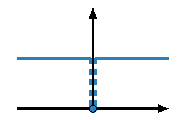
\includegraphics[width=\textwidth]{Figures/l0_regularizer.pdf}
         \caption{$\ell_0$}
     \end{subfigure}%
     \begin{subfigure}[b]{0.25\textwidth}
         \centering
         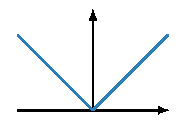
\includegraphics[width=\textwidth]{Figures/l1_regularizer.pdf}
         \caption{$\ell_1$}
     \end{subfigure}%
     \begin{subfigure}[b]{0.25\textwidth}
         \centering
         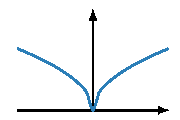
\includegraphics[width=\textwidth]{Figures/lh_regularizer.pdf}
         \caption{$\ell_p,\, p=1/2$}
     \end{subfigure}%
     \begin{subfigure}[b]{0.25\textwidth}
         \centering
         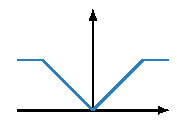
\includegraphics[width=\textwidth]{Figures/scad_regularizer.pdf}
         \caption{SCAD}
     \end{subfigure}
     \caption{Four commonly-used regularizers which promote sparsity}
     \label{fig:three graphs}
\end{figure}

\end{frame}

\begin{frame}{SR3-Relaxation for Mixed-Effect Models ($\ouralgo$)}
Original problem $\mathcal{FS-LME}$:
\eq{
	\min_{\beta \in \R^p,\, \gamma \in \R^{q}_+} \LL(\beta, \gamma) + R(\beta, \gamma)
}
Relaxed problem $\ouralgo$:
\eq{
	\label{eq:msr3_formulation_explicit}
	\min_{\beta, \tbeta \in \R^p,\, \gamma, \tgamma \in \R^{q}_+} \LL(\beta, \gamma) + \phi_\mu(\gamma) + \kappa_\eta(\beta - \tbeta, \gamma - \tgamma) + R(\tbeta, \tgamma)
}
where the \textit{relaxation} $\kappa_\eta$ decouples the likelihood and the regularizer 
\eq{
	\kappa_\eta(\beta - \tbeta, \gamma - \tgamma) := \frac{\eta}{2}\|\beta - \tbeta\|^2_2 + \frac{\eta}{2}\|\gamma - \tgamma\|_2^2, \quad \eta > \bar\eta
}
and the \textit{perspective mapping} $\phi_\mu$ replaces $\gamma \geq 0$ with a log-barrier 
\eq{
	\phi_\mu(\gamma) := \begin{cases}
		-\mu\sum_{i=1}^q \ln(\gamma_i/\mu), & \mu > 0 \\
		\delta_{\R_+^q}(\gamma), & \mu = 0 \\
		+\infty, & \mu < 0
	\end{cases}
} 
\end{frame}

\begin{frame}{Value Function Reformulation}
$\ouralgo$-relaxation replaces the original likelihood $\LL$ with a \textit{value function} $u_{\eta,\mu}$:
\eq{
	\label{eq:value_function_definition}
	u_{\eta,\mu}(\tbeta,\tgamma) & := \min_{(\beta, \gamma)} \LL_{\eta,\mu}((\beta, \gamma),(\tbeta, \tgamma)) \\  & := \min_{(\beta, \gamma)} \LL(\beta, \gamma) + \phi_\mu(\gamma) + \kappa_\eta(\beta - \tbeta, \gamma - \tgamma)
}
so $\ouralgo$-formulation~(\ref{eq:msr3_formulation_explicit}) becomes
\eq{
	\min_{(\tbeta, \tgamma) \in \CC} u_{\eta,\mu}(\tbeta, \tgamma) + R(\tbeta, \tgamma)
}
When $\eta$ is larger than the weak-convexity constant
\begin{itemize}
	\item $u_{\eta,\mu}$ is well-defined and continuously differentiable.
	\item As $\mu \rightarrow 0$ and $\eta \rightarrow \infty$, cluster points of solutions to $\ouralgo$ are first-order stationary points for $\mathcal{FS-LME}$ \\ 
\end{itemize}

\textbf{Key observation}: in practice, we don't need accurate solutions for~(\ref{eq:value_function_definition}): a few Newton iterations keep the solution close to the central path.
\end{frame}

\begin{frame}{Value Function Reformulation}
\begin{figure}
	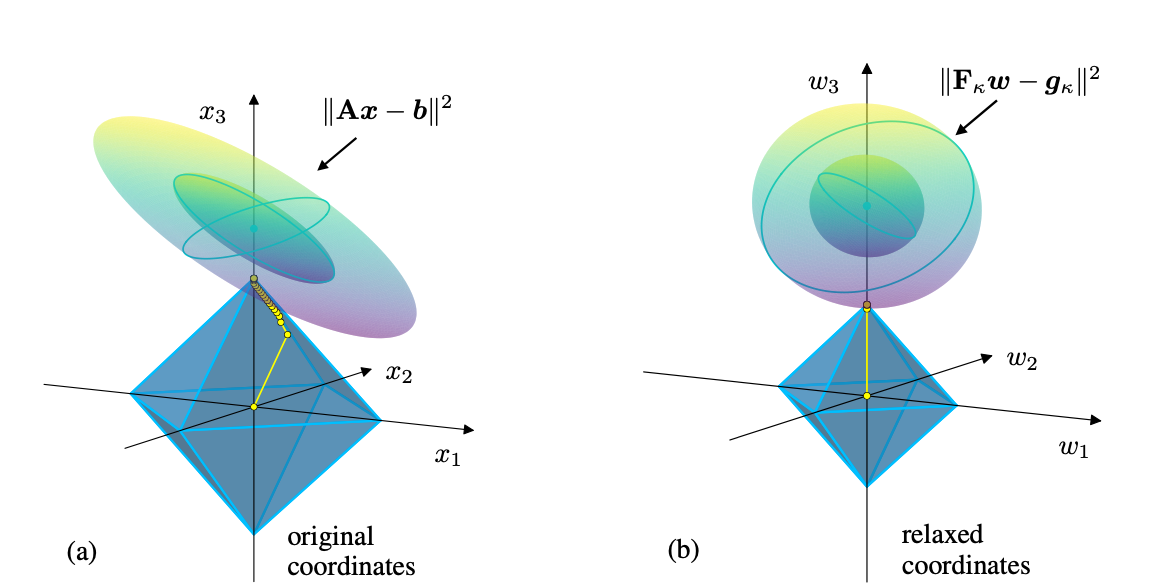
\includegraphics[width=\textwidth]{Figures/intuition_prev_paper}
	\caption{\label{fig:intuition_prev} Picture from \cite{Zheng2018RelaxAndSplit}: for a linear problem, value function relaxation ``squashes'' level-sets simplifying the optimization landscape.}
\end{figure}
\end{frame}

\begin{frame}{Value Function Reformulation}
\begin{figure}
	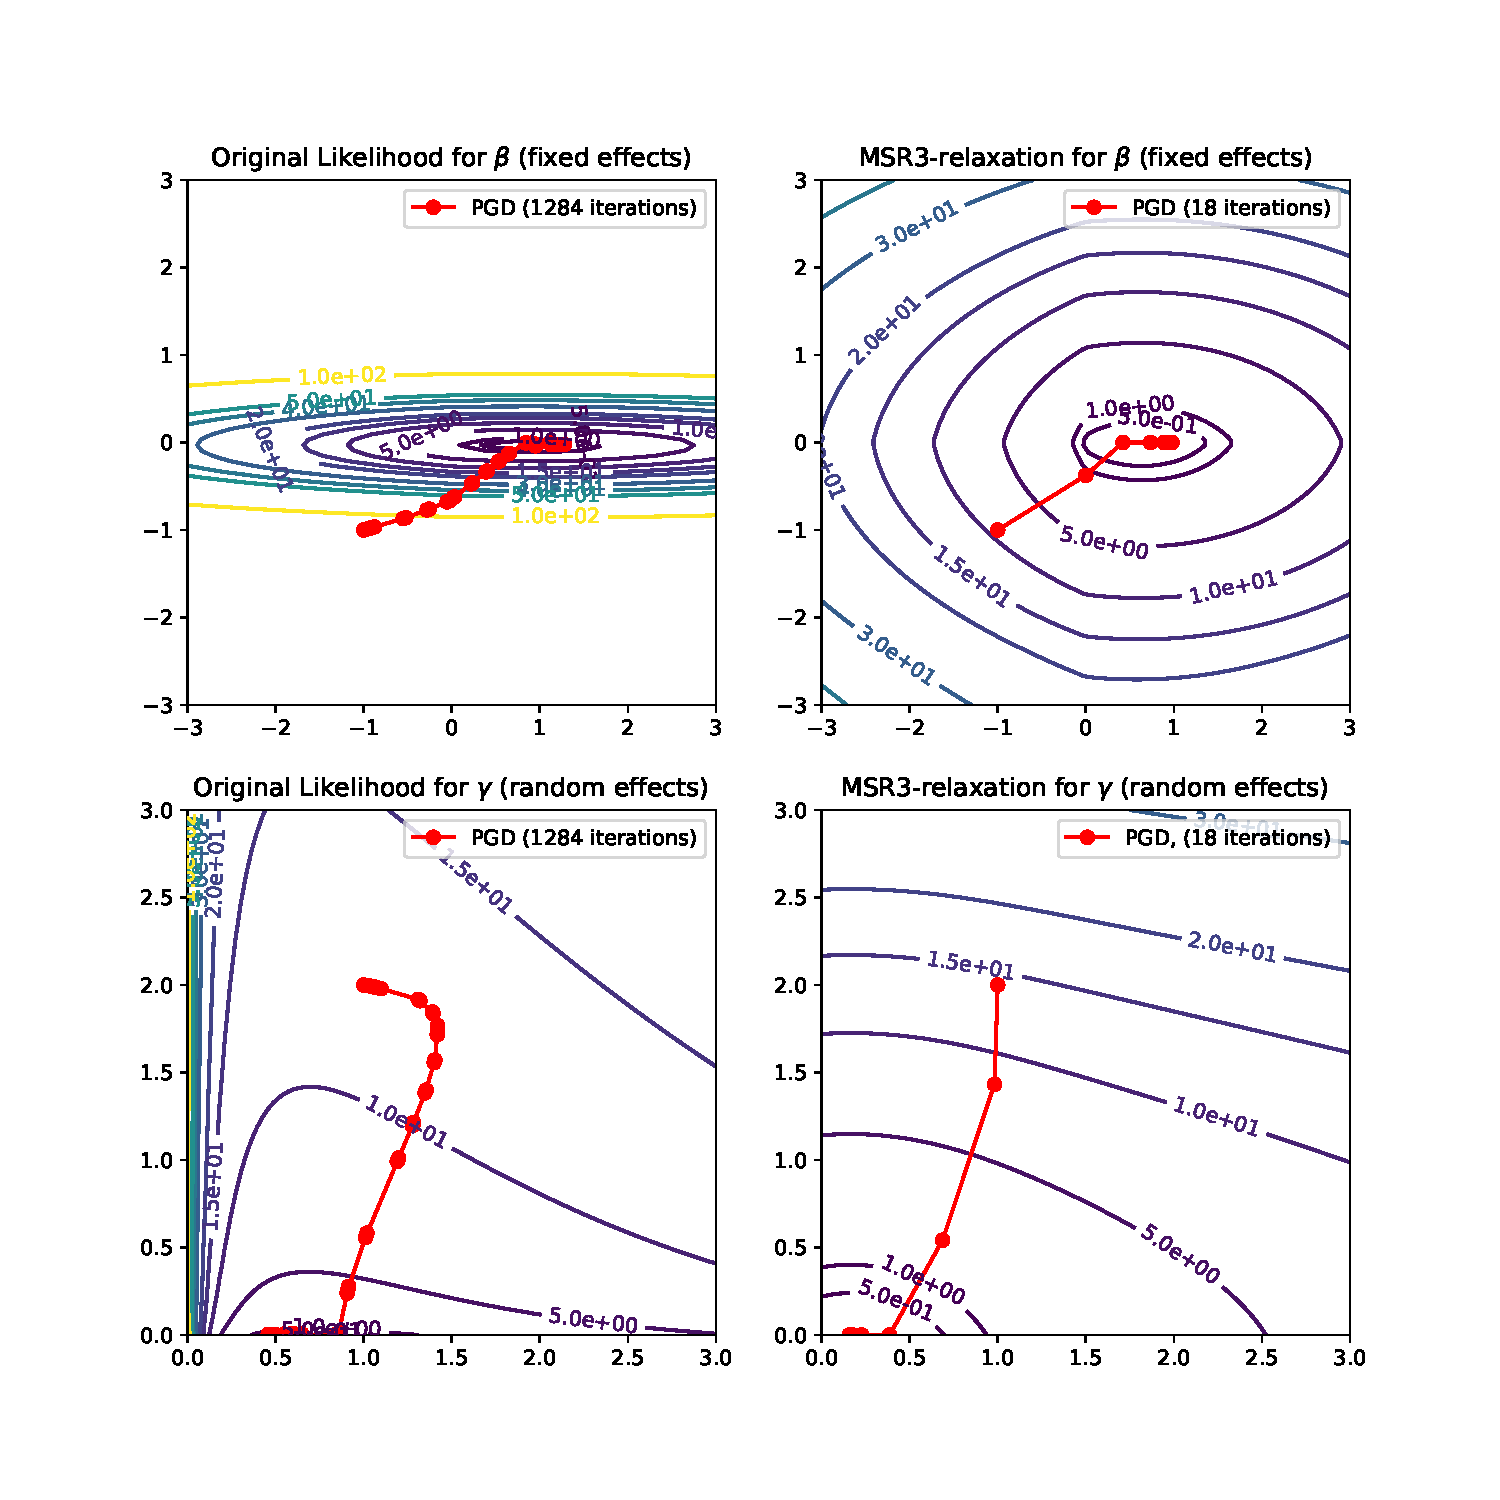
\includegraphics[width=0.7\textwidth]{Figures/intuition_current.pdf}
	\caption{\label{fig:intuition_sr3} Comparison of the level-sets for the original likelihood (left) and $\ouralgo$-likelihood (right), for fixed (top) and random (bottom) effects.}
\end{figure}
\end{frame}

\begin{frame}{Designing an Algorithm}
	$G_{\nu,\eta}$ encodes both gradient of a Lagrangian (lines 1-2) and the complementarity condition (line 3):
	\eq{
		G_{\nu,\eta}((\beta,\gamma,v),(\tbeta,\tgamma)) := \begin{bmatrix}
			\nabla_\beta \LL(\beta, \gamma) + \eta(\beta-\tbeta) \\
			\nabla_\gamma \LL(\beta, \gamma) + \eta(\gamma-\tgamma) - v\\
			v \bigodot \gamma - \mu\textbf{1}
		\end{bmatrix}
	}
	We apply Newton method to $G$ while geometrically decreasing $\mu$. \\
\textbf{Lemma:} For every $(\mu,\eta) \in \R_+\times\R_{++}$,
\eq{
	&(\hat\beta,\hat\gamma) = \argmin_{(\beta,\gamma)}\LL_{\eta,\mu}((\beta, \gamma),(\tbeta, \tgamma)) \\
	& \iff \\
	& \exists \hat{v} \in \R_{+}^q \text{ s.t. } G_{\nu,\eta}((\beta,\gamma,\hat{v}),(\tbeta,\tgamma)) = 0
}
If $\mu > 0$, then $\hat{v} = -\nabla\phi_\mu(\hat{\gamma})$, and if $\mu = 0$, then $\hat{v}$ is the unique KKT multiplier associated with the constraint $0 \leq \gamma$.
\end{frame}

\begin{frame}{$\ouralgo$-fast Algorithm}
\label{appendix:pseudocode}
\begin{algorithm}[H]
\SetAlgoLined
$\texttt{progress}\leftarrow \textbf{True}$; \quad \texttt{iter = 0}; \\
$\beta^+, \tbeta^+\leftarrow\beta_0$; 
\quad $\gamma^+, \tgamma^+\leftarrow\gamma_0$;  
\quad $v^+ \leftarrow 1 \in \R^q$; 
\quad  $\mu \leftarrow \frac{{v^+}^T\gamma^+}{10 q}$\\
 \While{\texttt{iter} $<$ \texttt{max\_iter}  \ and \ $\|G_\mu(\beta^+, \gamma^+, v^+)\|$ $>$ \texttt{tol}   \ and  \ \texttt{progress} \\}{
    $\beta \leftarrow \beta^+$; \quad $\gamma \leftarrow \gamma^+$; \quad $\tbeta \leftarrow \tbeta^+$; \quad $\tgamma \leftarrow \tgamma^+$ \\
%    $A \leftarrow \nbla G_\mu((\beta, \gamma, v), (\tbeta, \tgamma))$\\
  %  $b \leftarrow G_\mu((\beta, \gamma, v), (\tbeta, \tgamma))$\\
    $[dv, d\beta, d\gamma] \leftarrow  \nabla G_\mu((\beta, \gamma, v), (\tbeta, \tgamma))^{-1}  G_\mu((\beta, \gamma, v), (\tbeta, \tgamma))$
    $\alpha \leftarrow 0.99\times\min\left(1, -\frac{\gamma_i}{d\gamma_i}, \forall i :\ d\gamma_i < 0\right)$\\
    $\beta^+ \leftarrow \beta + \alpha d\beta$; \quad $\gamma^+ = \gamma + \alpha d\gamma$; \quad  $v^+ \leftarrow v + \alpha dv$\\
    \lIf{$\|\gamma^+\odot v^+ - q^{-1}{\gamma^+}^Tv^+ \mathbf{1}\| > 0.5q^{-1}{v^+}^T\gamma^+$}{continue}
    \Else{ 
        $\tbeta^+ = \prox_{\alpha R}(\beta^+)$;
        \    $\tgamma^+ = \prox_{\alpha R + \delta_{\R_+}}(\gamma^+)$; 
        \    $\mu = \frac{1}{10}\frac{{v^+}^T\gamma^+}{q}$
    }
%	\tcp*[h]{Keep iterating until convergence} \\
    \texttt{progress} = ($\|\beta^+ - \beta\| \geq \text{tol}$ or $\|\gamma^+ - \gamma\|  \geq \text{tol}$ or $\|\tbeta^+ - \tbeta\| \geq \text{tol}$ or $\|\tgamma^+ - \tgamma\| \geq \text{tol}$)\\
    \texttt{iter += 1}
 }
 \Return{$\tbeta^+$, $\tgamma^+$}
\end{algorithm}

\end{frame}

\section{Experiments}
\subsection{Application to Synthetic Problems}

\begin{frame}{Application to Synthetic Problems}
\textbf{The Experiment} 
\begin{itemize}
	\item The number of fixed effects $p$ and random effects $q$ is 20.
	\item $\beta = \gamma = \frac{1}{2}[1,2,3,\dots,10, 0\dots,0]$
	\item 9 groups with sizes [10, 15, 4, 8, 3, 5, 18, 9, 6]
	\item $X_i \sim \NN(0, I)^p$, $Z_i = X_i$, $\varepsilon_i \sim \NN(0, 0.3^2I)$
	\item Each experiment is repeated 100 times.
	\item Grid-search for $\eta \in [10^{-4}, 10^{2}]$, golden search for $\lambda \in [0, 10^5]$
	\item Final model is chosen to maximize BIC
\end{itemize}
\begin{table}
	\begin{tabular}{lllll}
\toprule
     & Model &    PGD &    MSR3 & MSR3-fast \\
Regularizer & Metric &        &        &       \\
\midrule
L0 & Accuracy &   0.89 &   \textbf{0.92} &  \textbf{0.92} \\
     & Time &  41.68 &  88.54 &  \textbf{0.13} \\
L1 & Accuracy &   0.73 &   \textbf{0.88} &  \textbf{0.88} \\
     & Time &  38.39 &   9.13 &  \textbf{0.13} \\
ALASSO & Accuracy &   0.88 &   \textbf{0.92} &  0.91 \\
     & Time &  34.55 &  65.19 &  \textbf{0.12} \\
SCAD & Accuracy &   0.71 &   \textbf{0.93} &  0.92 \\
     & Time &  77.62 &  84.67 &  \textbf{0.17} \\
\bottomrule
\end{tabular}

\end{table}
\end{frame}

\begin{frame}{Application to Synthetic Problems}
\begin{figure}
	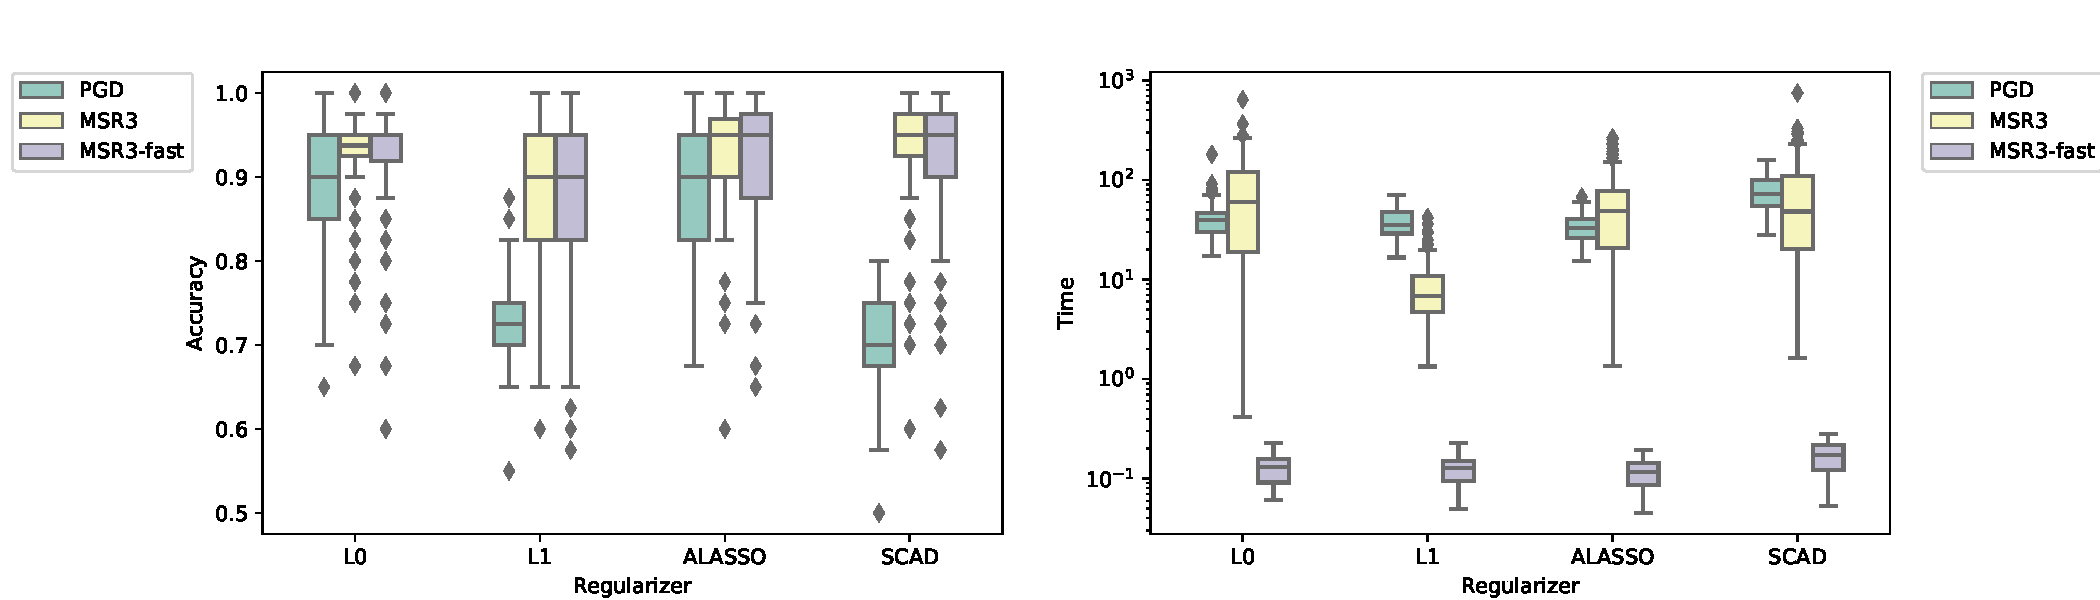
\includegraphics[width=\textwidth]{Figures/performance_picture_current.pdf}
\end{figure}
Benefits:
\begin{itemize}
	\item $\ouralgo$-relaxation improves feature selection performance than the original likelihood.
	\item $\ouralgo$-fast optimization accelerates the compute time by $\sim 10^2$.
\end{itemize}
Challenge:
   \begin{itemize}
   	\item Initialization of $\eta$ is problem-specific
   \end{itemize}
\end{frame}

\begin{frame}{Choice of $\eta$}
	\begin{figure}
		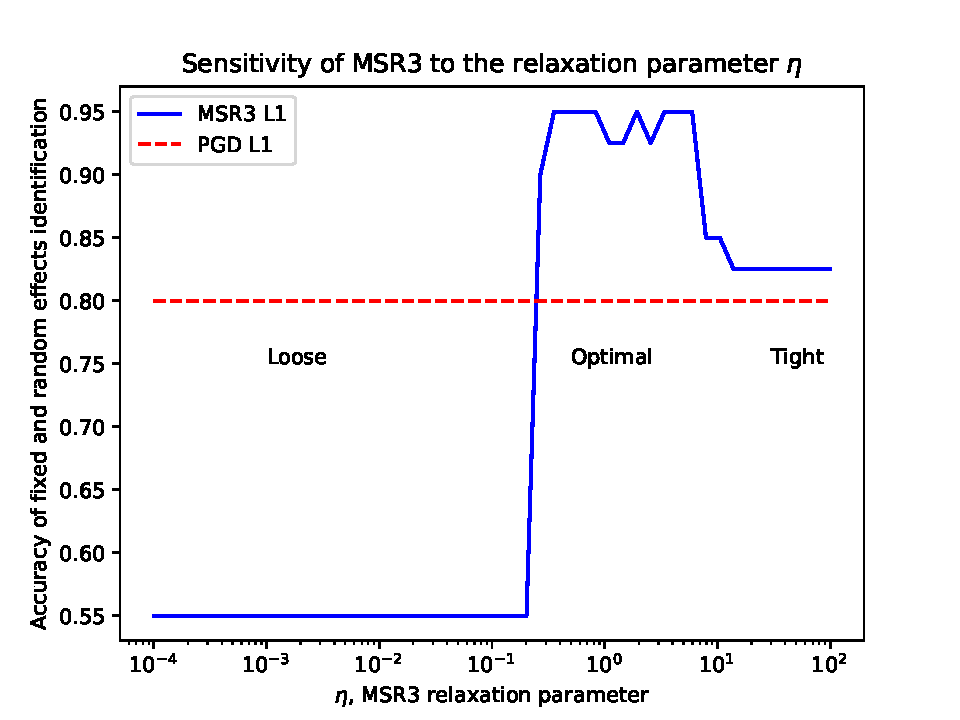
\includegraphics[width=\textwidth]{Figures/eta_L1.pdf}
	\end{figure}
\end{frame}

\begin{frame}{$\ell_0$-based Covariate Selection for Bullying Study from GBD}
	\begin{figure}
		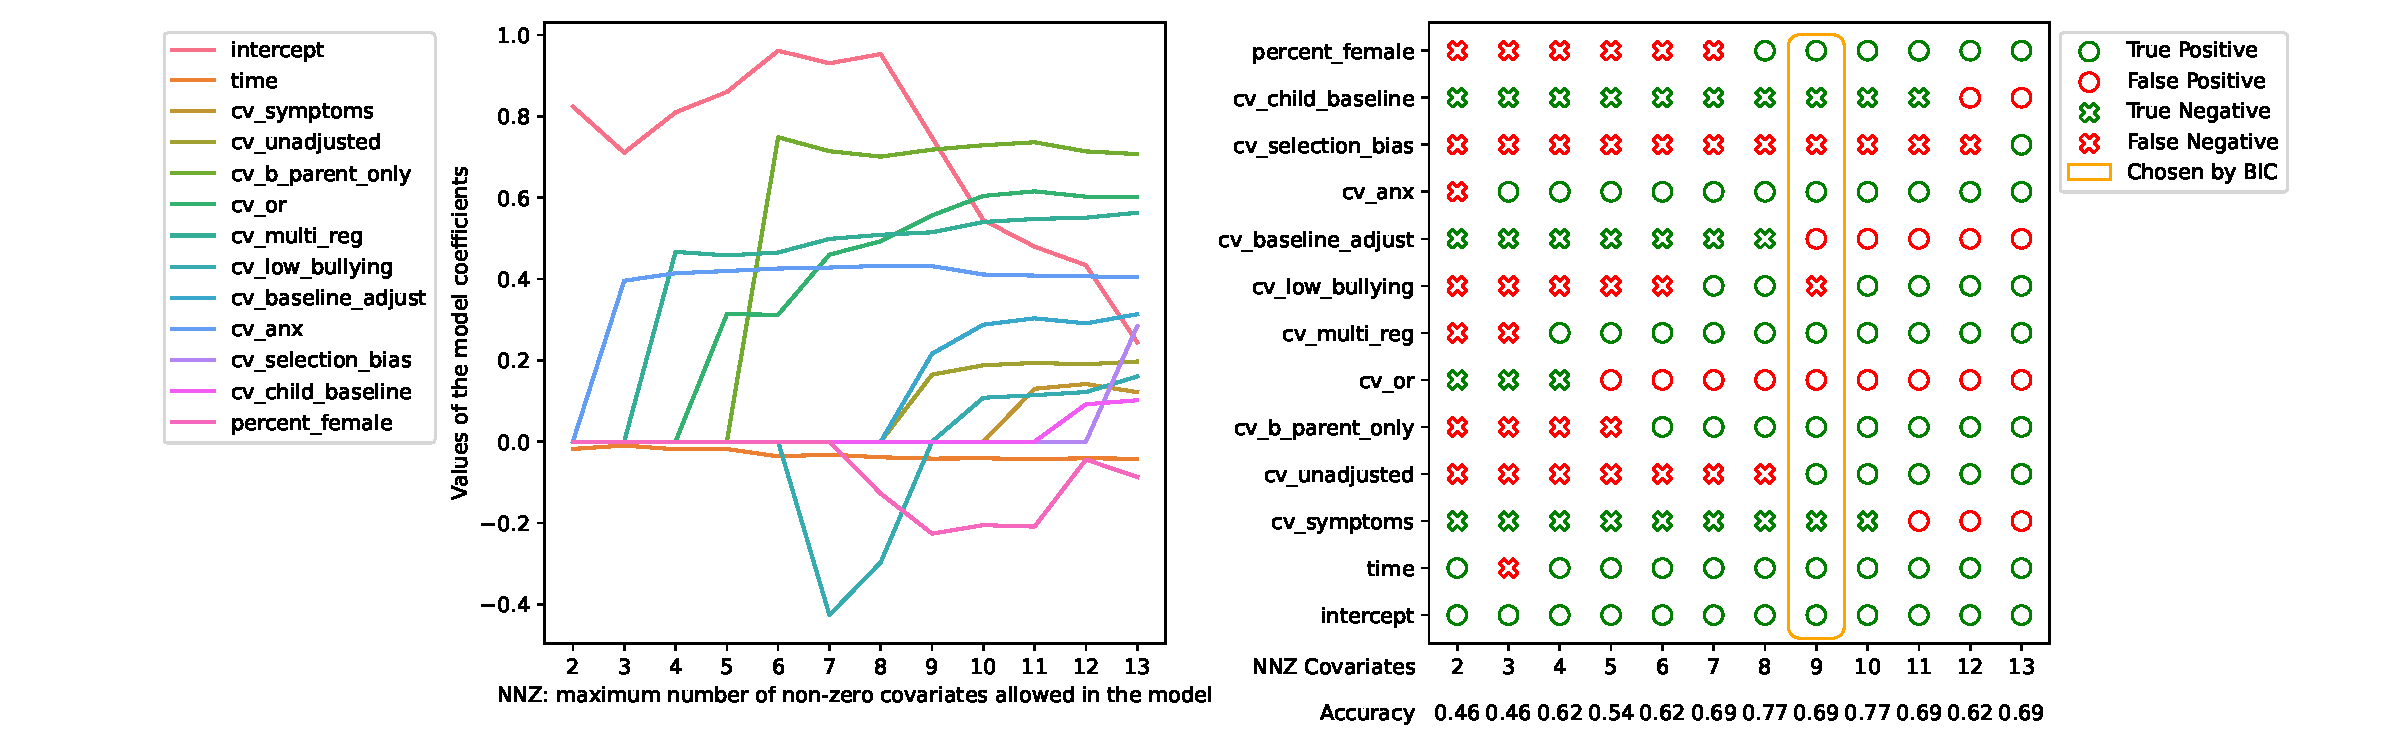
\includegraphics[width=\textwidth]{Figures/bullying_data_assessment_selection.pdf}
		\caption{Fixed and random covariate selection for Bullying dataset from~\cite{GBD}. The model selected 9 covariates, 7 of which were historically significant, and did not select 4 covariates, 1 of which was historically significant.}
	\end{figure}
\end{frame}

\begin{frame}{Thank You!}
	The code is available on GitHub: \href{github.com/aksholokhov/pysr3}{https://github.com/aksholokhov/pysr3}
	\begin{itemize}
		\item All estimators are fully compatible to \texttt{sklearn} library.
		\item Implements SR3 for linear, generalized-linear, and linear mixed-effect models.
		\item Has tutorials, tests, and documentation.
	\end{itemize}
\end{frame}
\begin{frame}{References}
	\textbf{References}: 
	\bibliographystyle{plain}
	\bibliography{bibliography.bib}
\end{frame}

\end{document}